\section{SLAM}

We don't really have too many results to show in regards to the SLAM, as we don't get to test it on anything else than simulator until the car is ready, which is going to be some time after this project thesis is delivered. 

Possible things I can plot:
\begin{itemize}
    \item runtime? Maybe both frontend and backend in one plot?
    \item Map error compared with ground truth as a function of detection noise? Much work \:(
    \item Size of hypotheses-list over time?
\end{itemize}

When simulating with false positives generated with a random gaussian position, the frontend doesn't let any false positives through. This is of course not the best metric for performance, since detection systems don't really send false positives with completely random position. The ones they send are usually because of objects around the track, like walls, and will be spatially correlated. This means that the frontend will have to deal with false positives that cluster around partiular areas. Detection data from last year shows that the false positives that get detected usually jump around a lot, so hopefully the frontend will spawn many new hypotheses that loose confidence, instead of associating to the same false positive and evntually sending it through to the backend. This is not possible to test at the moment unfortunately, since the data from last year isn't compatible with the current system. 

\begin{figure}
    \centering
    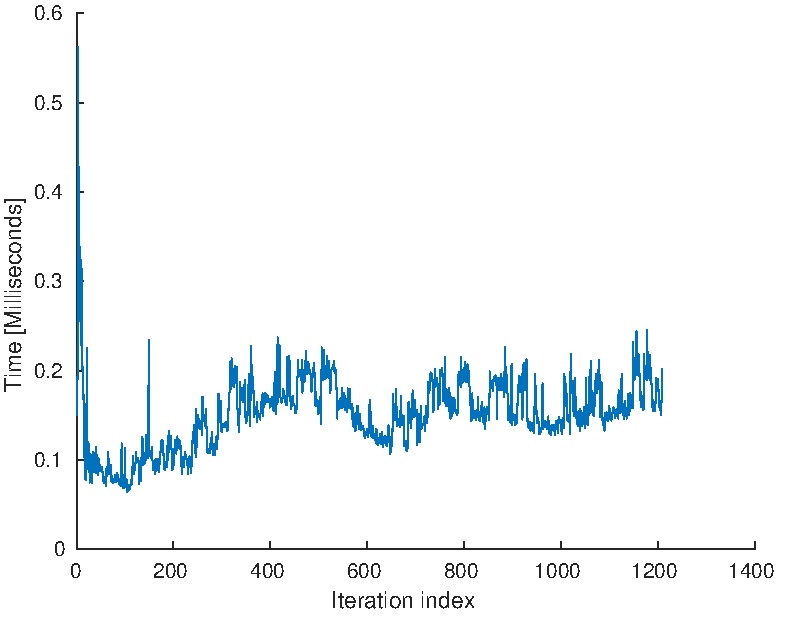
\includegraphics[width=0.8\linewidth]{0_Images/6_Results/FrontendTiming.pdf}
    \caption[Runtime of the SLAM frontend.]
    {Runtime of the SLAM frontend over time, when simulating with gaussian noise on detection and odometry. The timing is from when the set of detection arrives from one of the detection systems to when it is done processing. Simulated using the track from FSG's Autocross event 2018.}
    \label{Fig:FrontendTiming}
\end{figure}

\begin{figure}
    \centering
    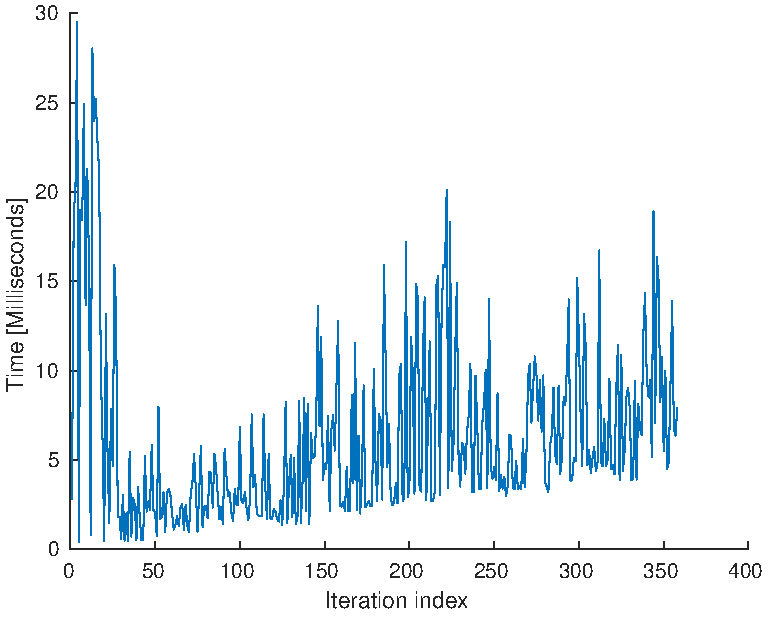
\includegraphics[width=0.8\linewidth]{0_Images/6_Results/BackendTiming.pdf}
    \caption[Runtime of the SLAM backend.]
    {Runtime of the SLAM backend over time, for one complete update. One update means adding all the new information to the graph, optimizing the graph and then sending out the map and pose correction. Simulated using the track from FSG's Autocross event 2018.}
    \label{Fig:BackendTiming}
\end{figure}

\begin{figure}
    \centering
    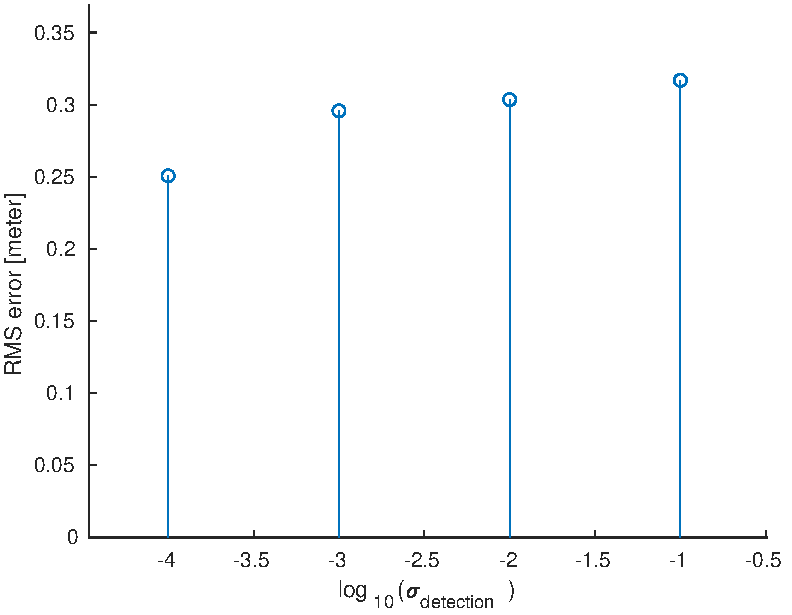
\includegraphics[width=0.8\linewidth]{0_Images/6_Results/SLAMERMS.pdf}
    \caption[SLAM RMS error as a function of logarithm of the standard deviation on the noise added to the detections.]
    {SLAM RMS error as a function of logarithm of the standard deviation on the noise added to the detections. Simulated on one full round around the FSG autocross event 2018. Simulated ten times for each value of the standard deviation and the mean of the rms errors was taken.}
    \label{Fig:SLAMERMS}
\end{figure}